\section{Results}\label{results}
In this section we describe the results.

\subsection{Benchmarking}

\begin{figure}[!ht]
  \centering
    \includegraphics[width=0.67\textwidth]{../figs/gfedComparison.png}
  \caption{Benchmark comparisons against GFED4s \citep{Giglio2013}.}
\end{figure}

\subsection{Limitations}

\begin{figure}[!ht]
  \centering
    \includegraphics[width=0.67\textwidth]{../figs/limitation_lines.png}

  \caption{Limitation covers.}
\end{figure}


\subsection{Sensitivity}

\begin{figure}[!ht]
  \centering
    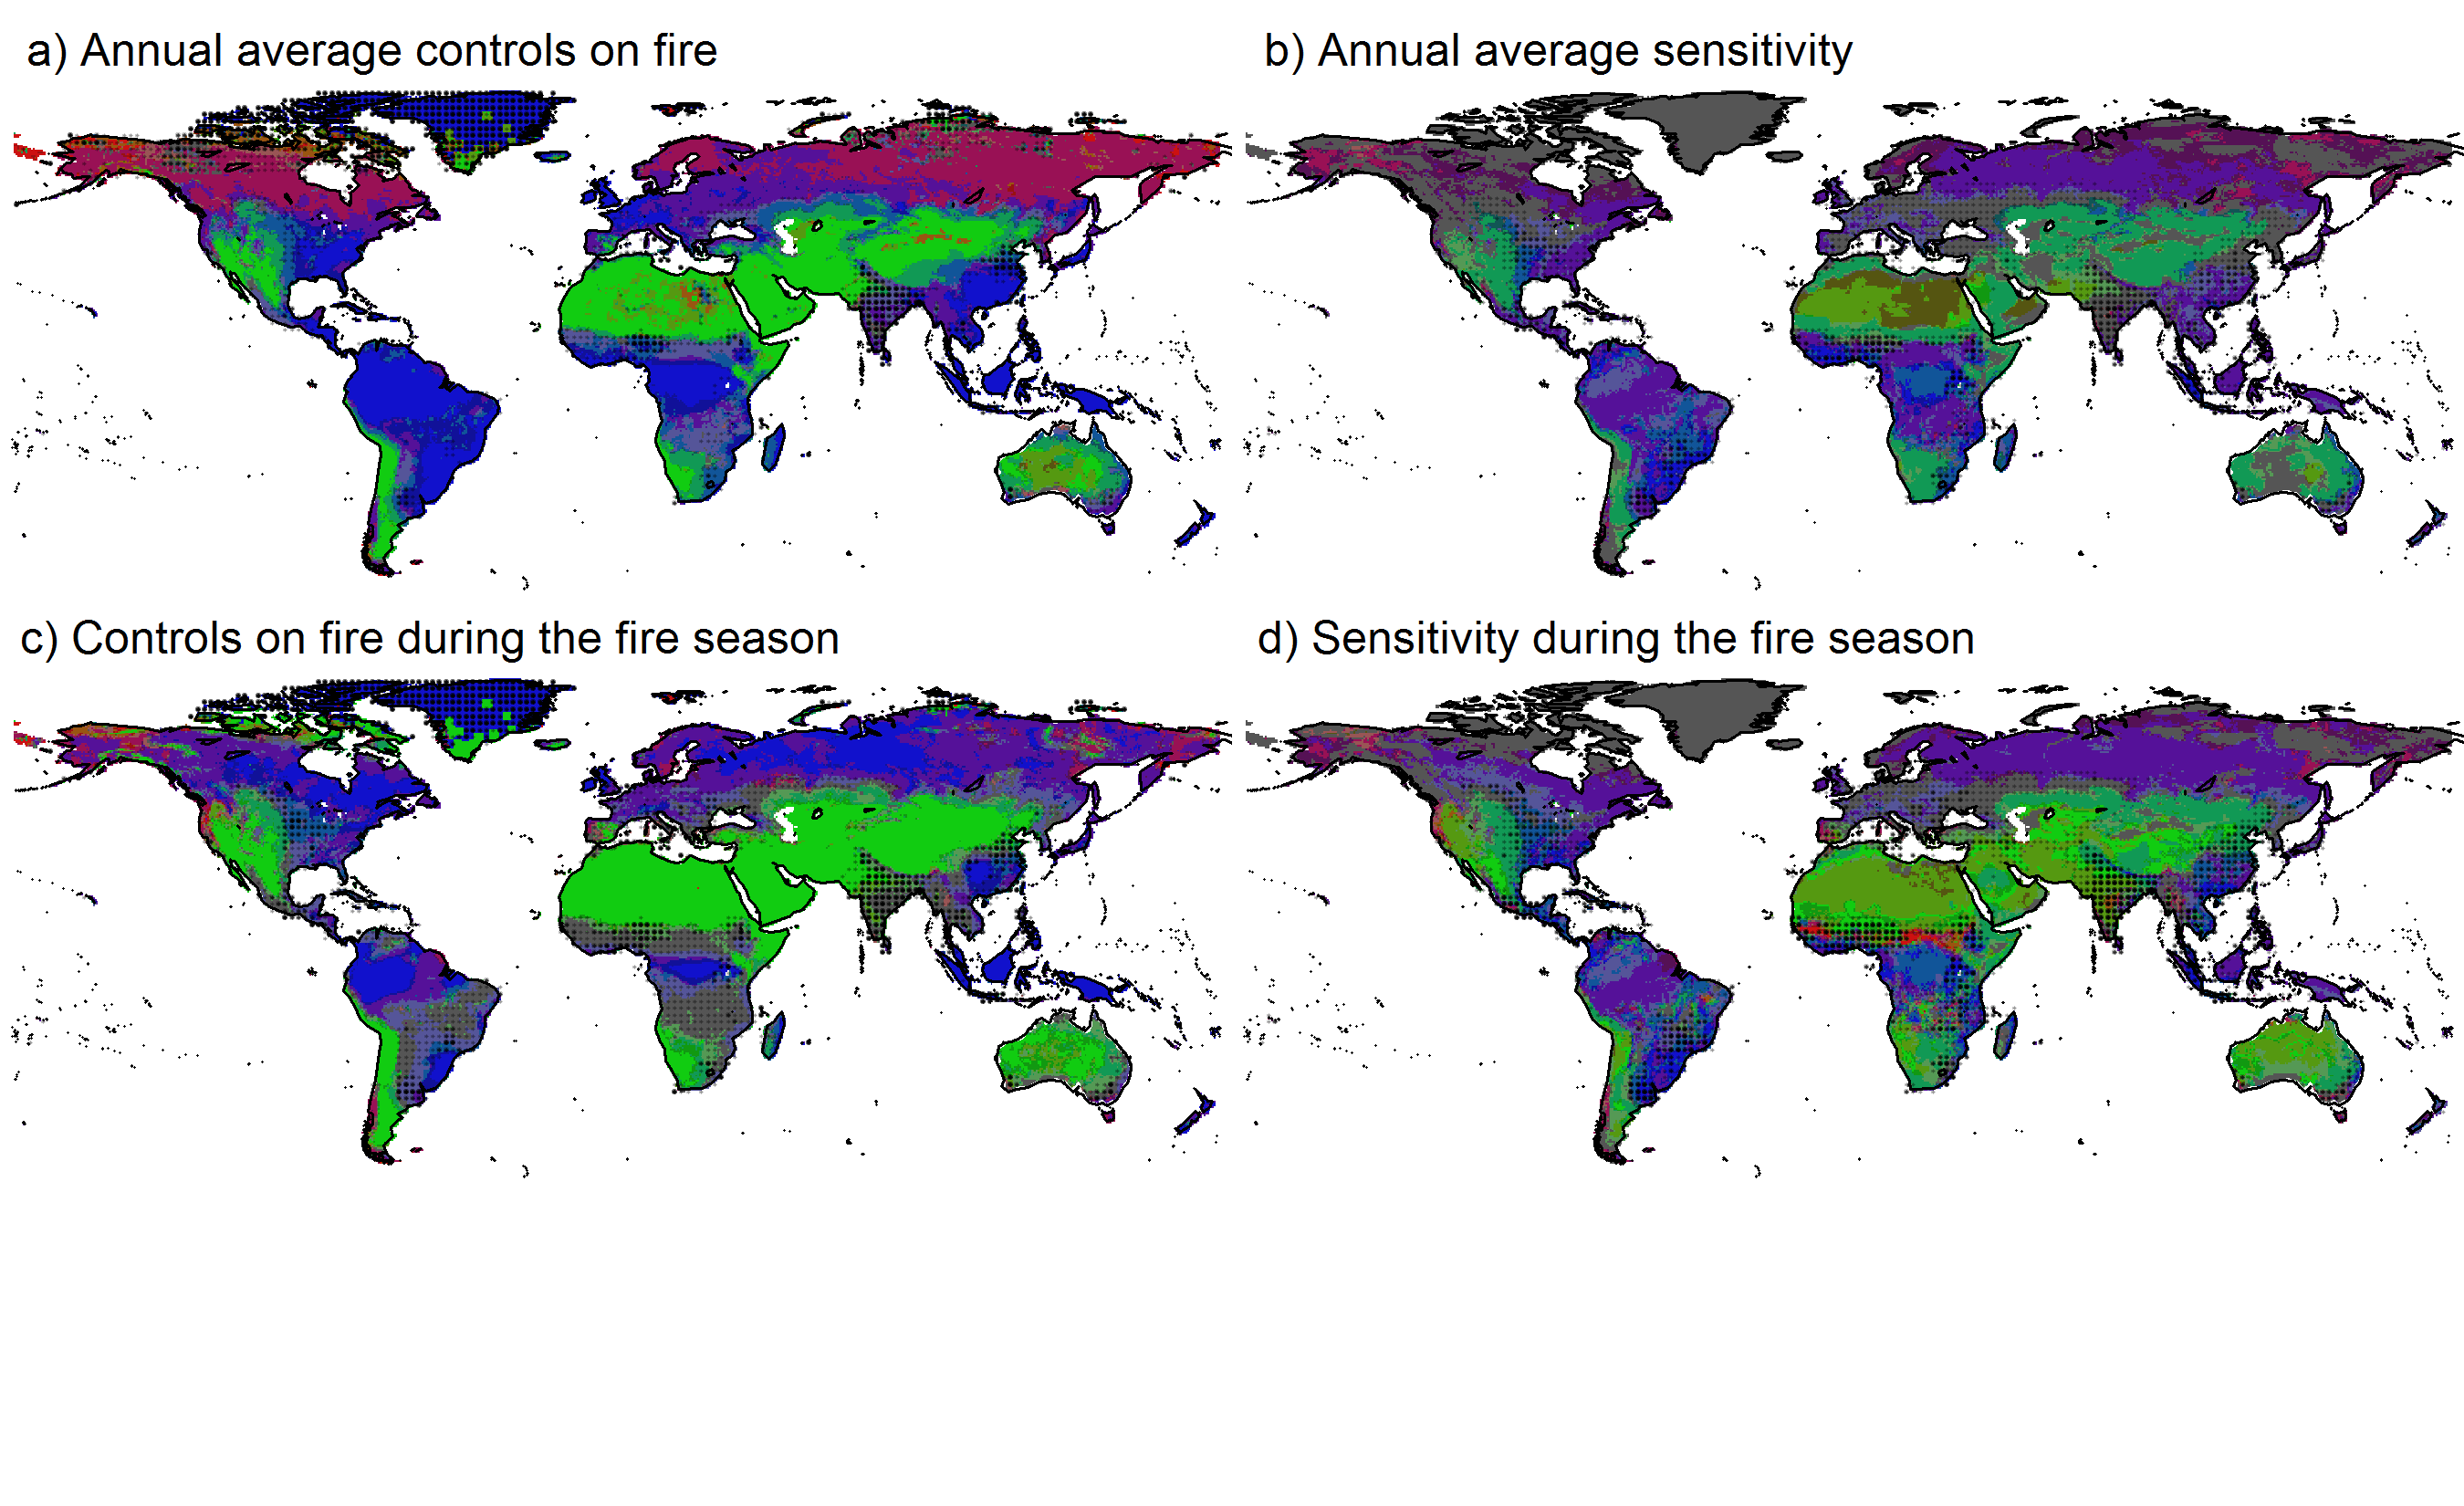
\includegraphics[width=0.67\textwidth]{../figs/limitation_map.png}

  \caption{Limitation and sensitivity.}
\end{figure}

\begin{figure}[!ht]
  \centering
    \includegraphics[width=0.67\textwidth]{../figs/moisture_change_for_Amazon_tipping_point.png}

  \caption{Required change in \% fuel moisture content to induce savanna-level fire in the Amazon.}
\end{figure}


\subsection{Human impact}

\begin{figure}[!ht]
  \centering
    \includegraphics[width=0.67\textwidth]{../figs/HumanImpactMap_small.png}

  \caption{Human impact on burnt area.
            a) Increases in burnt area from human induced fire starts.
            b) Changes in burnt area from human fire starts and supression.}
\end{figure}

